\section{Lecture 8}
\textbf{Gordon Newell QNs:} always stable.

\hrule
\settowidth{\MyLen}{\texttt{Service Demand.}}
\begin{tabular}{@{}p{\the\MyLen}@{}p{\linewidth-\the\MyLen}@{}}
\verb!Visit count!	&  $V_j = \sum^M_{i=1} V_ir_{i,j}$, Solavble if one of the Vs is given\\
\verb!Service Demand!	&  $D_i = V_i \cdot E[S_i]$. Highest service demand is bottleneck\\
\end{tabular}
\hrule
If we increase K, then $X(K) \rightarrow \frac{1}{D_b}$ and $\rho_b \rightarrow 1$. For non-bottleneck stations, $\rho_i \rightarrow \frac{D_i}{D_b} < 1$

\textbf{Gordon And Newell product-form:} $I(M,K)$ is every possible combination of $\underline{n} = (n_1, n_2 ... n_M)$. $P(\underline{N} = \underline{n}) = \frac{1}{G(M,K)} \prod^M_{i=1} D_i^{n_i}$ with normalisation constant $G(M,K) = \sum_{n \in I(M,K)} \prod_{i=1}^M D_i^{n_i}$. Size of $I(M,K) = {M+K-1 \choose M-1}$

\textbf{MVA:} 

\hrule
\settowidth{\MyLen}{\texttt{2nd factorial moment.}}
\begin{tabular}{@{}p{\the\MyLen}@{}p{\linewidth-\the\MyLen}@{}}
$E[\hat{R}_i(k)]$ 	&  $(E[N_i(k-1)] + 1)D_i$\\
$E[\hat{R}(k)]$ 	&  $\sum E[\hat{R}_i(K)]$\\
$X(K)$ 				&  $\frac{K}{E[\hat{R}(k)]}$\\
$E[N_i(k)]$ 		&  $X(k)E[\hat{R}_i(k)]$\\
\verb!For IS node!  &  $E[R_i](K) = E[S_i]$ and $E[\hat{R}_i](K) = D_i$
\end{tabular}
\newline
\hrule
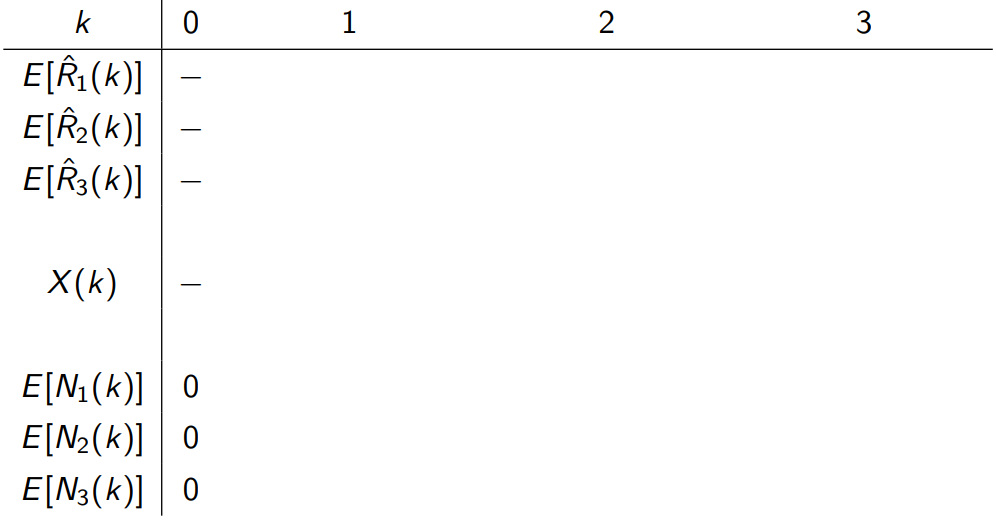
\includegraphics[scale=0.2]{images/MVA.png}

\textbf{Asumptotic bounds:}
\hrule
\settowidth{\MyLen}{\texttt{Saturation point.}}
\begin{tabular}{@{}p{\the\MyLen}@{}p{\linewidth-\the\MyLen}@{}}
\verb!X(K) upperbound! 	&  $X(K) \leq \min\{\frac{K}{E[Z] + D_\Sigma}, \frac{1}{D_+}\}$\\
\verb!E[R] lower bound! 	&  $E[\hat{R}(K)] \geq \max\{E[Z] + D_\Sigma, KD_+\}$\\
\verb!! 	&  \\
\verb!Saturation point! 	&  $K^*  = \frac{D_\Sigma + E[Z]}{D_+}$\\
\end{tabular}
\hrule

\textbf{Bard-Schweiter Approximation:}
MVA with $E[\hat{R}_i(K)] \approx (\frac{K-1}{K} E[N_i(K)] + 1) D_i$ and as a first guess $E[N_i](k) = \frac{K}{M}$.

\textbf{Balanced Queueing Networks:} Assume all station ahve the same service demands and $E[N_i(K)] = \frac{K}{M}$.
\hrule
\settowidth{\MyLen}{\texttt{Saturation point.}}
\begin{tabular}{@{}p{\the\MyLen}@{}p{\linewidth-\the\MyLen}@{}}
$E[\hat{R}_i(K)]$ 	&  $\frac{D(K+M-1)}{M}$\\
$E[\hat{R}_(K)]$ 	&  $D(K+M-1)$\\
$X(K)$ 	&  $\frac{K}{D(K+M-1)}$\\
$\rho_i(K)$ 	&  $\frac{K}{K+M-1}$\\
\verb!Simple bounds! 	&  \\
			& $\frac{K}{D_+(K+M-1)} \leq X(K) \leq \frac{K}{D_-(K+M-1)}$\\
			& $D_-(K+M-1) \leq E[\hat{R}(K)] \leq D_+(K+M-1)$\\
\verb!Tighter bounds! 	&  \\

\end{tabular}
\hrule
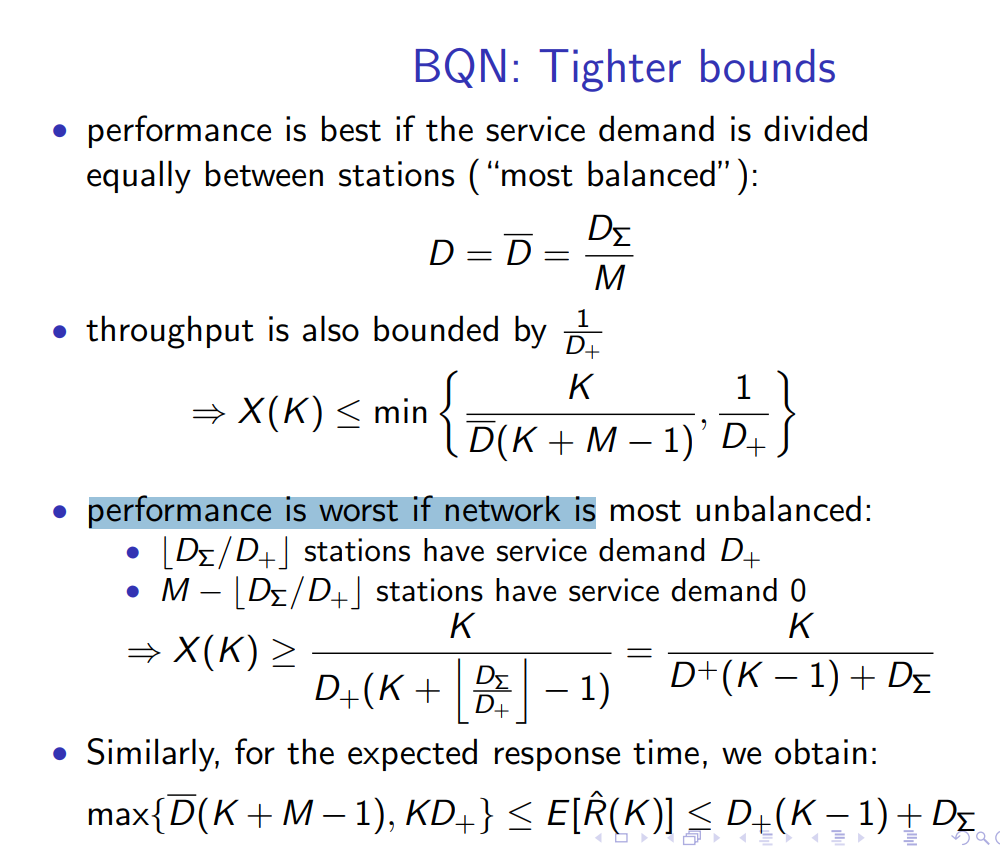
\includegraphics[scale=0.2]{images/geen_zin_meer.png}